\scanpage{32}
partie du même type. Par exemple toute intersection de feuilles fermées est une réunion de feuilles fermées.

La relation d'inclusion entre feuilles fermées induit une relation d'ordre sur l'ens des feuilles, appelée ``relation d'incidence''. La réunion des feuilles incidentes à une feuille donnée $F$ et distinctes d'elle n'est autre que $\overline F-F$; on l'appelle le \uline{bord} de la feuille $F$; c'est \unsure{bien|donc} une partie fermée, réunion de feuilles fermées.

\uline{Proposition} Pour que la filtration donnée de $X$ soit équisingulière, il f. et s. qu'elle satisfasse les 2 conditions:

a) $\forall$ feuille $F$, $\overline F$ est une réunion de feuilles

b) Le diagramme formé de $X$ et de toutes les feuilles fermées (avec les applications d'inclusion) est \deleted{\unsure{constant près de|constant par le}} \inserted{équisingulier} le long de chaque feuille.

On dit qu'une partition $(F_i)_{i\in I}$ \deleted{de $X$} \inserted{d'un} espace $X$ \inserted{en ``feuilles'' $F_i$} est \deleted{\unsure{équi}} une \uline{partition équisingulière} si 1°) chaque $F_i$ est la différence de deux sous-espaces fermés (i.e. $\overline{F_i}$ et $\overline{F_i}-F_i=bF_i$ sont des sous-espaces fermés) 2°) Chaque $\overline{F_i}$ est une réunion de feuilles et 3°) le diagramme formé par \inserted{$X$,} les $\overline{F_i}$ et leurs inclusions est équisingulier le long de chaque feuille.
\margin{Si 1° et 2° sont satisfaites on dira que la partition est cellulaire}
\figure{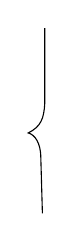
\begin{tikzpicture}\draw (0,0)--(-.02,.7)..controls(-.02,.9)and(-.1,1)..(-.18,1.02)..controls(-.02,1.1)and(.02,1.2)..(.03,1.4)--(.03,2.35);\end{tikzpicture}}
\mspage{33}
